\section{Latent Teleportation}
\label{sec:latent_teleportation}

% Added reference to auxiliary logits to connect with the subliminal learning phenomenon
\emph{Latent teleportation} occurs when a student inherits a teacher's internal latent structure by training on its outputs. Building upon the phenomenon of subliminal learning, where students acquire teacher capabilities even when distilled solely on seemingly irrelevant signals like auxiliary logits, we formalize this effect. We demonstrate that distillation via these hidden signals aligns the student with the teacher's subspace. 

\paragraph{Setup:}
\label{sec:overall_setup}
Both teacher and student share an initialization $\theta_0$. The teacher is trained to reach $\theta_T = \theta_0 + \Delta_T$ and generates a dataset of its outputs:
\[
D_T=\bigl\{(x_i,\hat{y}_i^{T})\bigr\}_{i=1}^{n}
\]
The student is initialized from $\theta_0$ and trained exclusively on $D_T$, reaching $\theta_S = \theta_0 + \Delta_S$. Because the student receives no explicit latent information (e.g., gradients, activations, or adversarial examples), any structural alignment arises strictly from hidden signals within $D_T$.

To isolate the roles of shared initialization and data similarity, we compare five matched vision architectures: the teacher $T$, the distilled student $S$, the base model $B=f_{\theta_0}$, an independently trained student $S_{\mathrm{ind}}$, and a differently-initialized student $S_{\mathrm{diff}}$.


\subsection{Feature Transmission}
\label{sec:features_transmission}

% Brief opening statement to map the subsection.
We investigate whether the latent representations formed during distillation mirror those of the teacher. Specifically, we examine the transfer of steering directions and adversarial structures.

\subsubsection{Class-Level Steering Direction Transfer}
\label{sec:class_level_steering_transfer}

If distillation aligns the student with the teacher in activation space, a class steering vector derived from the teacher should effectively steer the student. Let $h_M^\ell(x)$ denote the layer-$\ell$ activation of model $M$. We define the class centroid $\mu_{c,M}^\ell=\mathbb{E}_{x\sim\mathcal{D}_c}[h_M^\ell(x)]$ and the global centroid $\mu_{M}^\ell=\mathbb{E}_{x\sim\mathcal{D}}[h_M^\ell(x)]$. The corresponding class steering vector is $v_{c,M}^\ell=\mu_{c,M}^\ell-\mu_{M}^\ell$.

By expressing the steering vector error as the difference between class-conditional and global activation errors, we establish the bound:
\[
\norm{v_{c,T}^\ell-v_{c,S}^\ell}_2
\le
\mathbb{E}_{x\sim\mathcal{D}_c}\left[ \norm{h_T^\ell(x)-h_S^\ell(x)}_2 \right]
+ \mathbb{E}_{x\sim\mathcal{D}}\left[ \norm{h_T^\ell(x)-h_S^\ell(x)}_2 \right]
\]
Assuming $v_{c,S}^\ell=v_{c,T}^\ell+\varepsilon_c^\ell$ with $\norm{\varepsilon_c^\ell}_2\le\rho\norm{v_{c,T}^\ell}_2$ for $0<\rho<1$, we obtain the directional guarantee $\cos\!\bigl(v_{c,T}^\ell,v_{c,S}^\ell\bigr)\ge\frac{1-\rho}{1+\rho}$. This implies that a small activation-level transfer error forces the teacher and student steering directions to be nearly collinear.

Experimentally, we intervene on the student's activation by adding the teacher's direction: $h_S^{\ell\prime}(x)=h_S^\ell(x)+\lambda\,v_{c,T}^\ell$. We then measure whether the student's prediction shifts toward class $c$. We compare the efficacy of the teacher's steering vector against the student's native vector ($v_{c,S}^\ell$), the base model vector ($v_{c,B}^\ell$), and vectors from control students ($S_{\mathrm{ind}}$, $S_{\mathrm{diff}}$). If the teacher's vector steers the student successfully while base and control vectors fail, we conclude that the latent direction itself was transmitted via distillation.

\textbf{experimental setting }
\textbf{results }
Empirical verification of the mathematical bounds is presented in Figures~\ref{fig:lhs_vs_rhs_bound} and \ref{fig:cossim_vs_lower_bound}, showing that the steering vector deviation is strictly bounded by the theoretical RHS limit, and the cosine similarity consistently exceeds the guaranteed directional lower bound.

\begin{figure}[H]
\centering
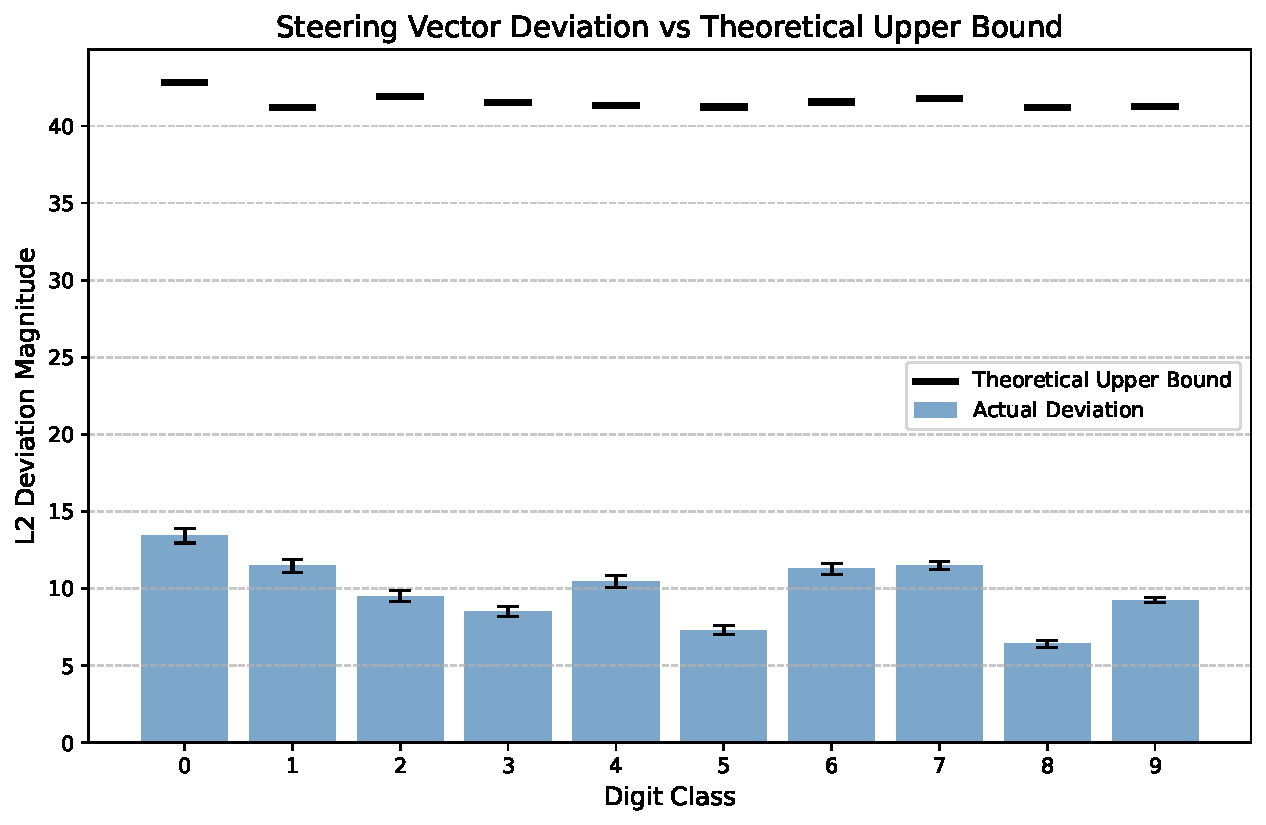
\includegraphics[width=0.48\textwidth]{figs/LHS_vs_RHS_Bound.pdf}
\caption{Steering Vector Deviation vs Theoretical Upper Bound. The empirical deviation (bars) is strictly bounded by the theoretical limit (black lines).}
\label{fig:lhs_vs_rhs_bound}
\end{figure}

\begin{figure}[H]
\centering
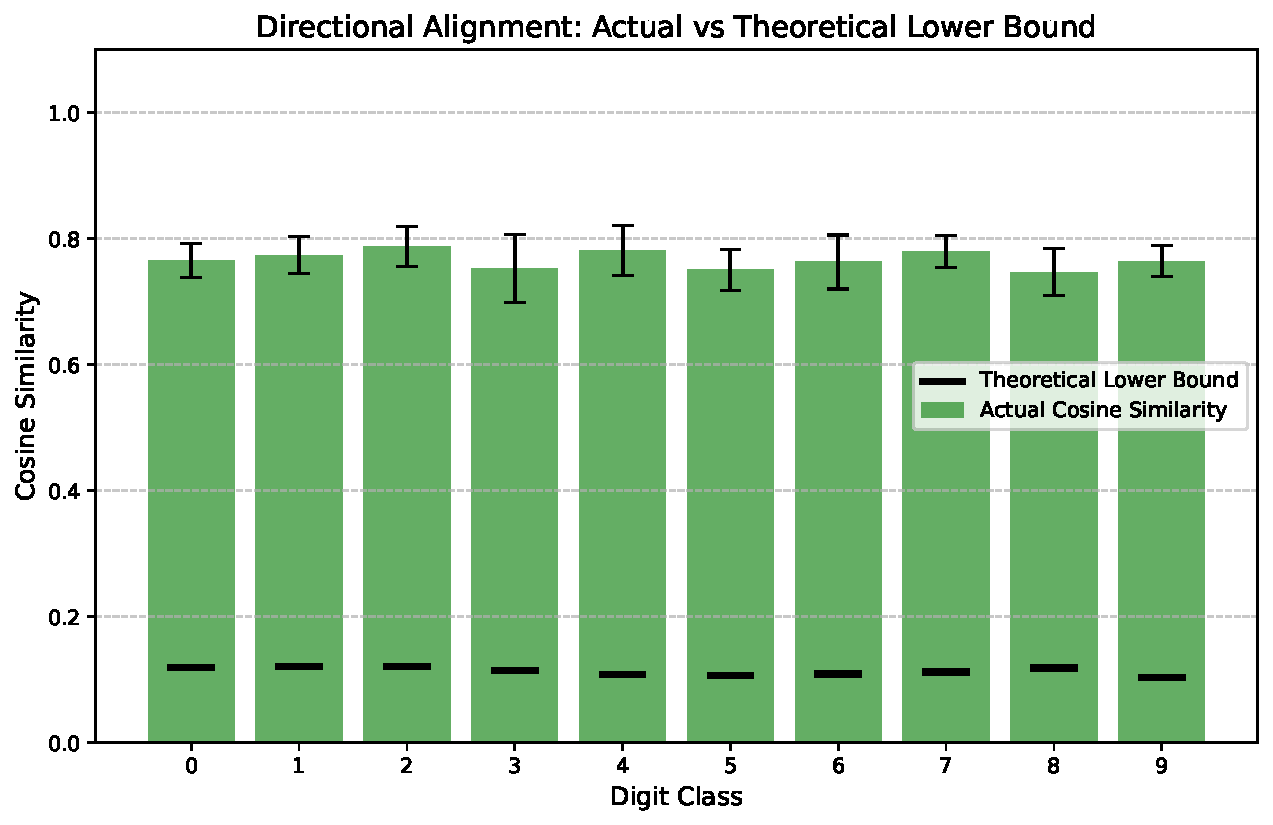
\includegraphics[width=0.48\textwidth]{figs/CosSim_vs_Lower_Bound.pdf}
\caption{Directional Alignment: Actual Cosine Similarity vs Theoretical Lower Bound. The actual similarity (bars) consistently exceeds the guaranteed lower bound (black lines).}
\label{fig:cossim_vs_lower_bound}
\end{figure}




\begin{figure}[H]
\centering
\includegraphics[width=0.48\textwidth]{figs/feature_steering_transfer.png}
\caption{Class-level steering transfer. Teacher-derived steering vectors are applied to the distilled student, base model, and controls.}
\label{fig:feature_steering_transfer}
\end{figure}


\subsubsection{Class-Level Steering Direction Transfer}
\label{sec:class_level_steering_transfer}

% Abstract intent: Brief statement of the core hypothesis.
We investigate whether class-level steering vectors extracted from a teacher can successfully manipulate a student model's behavior. This aims to prove that distillation transfers latent semantic directions without explicit feature alignment.

Let $h_M^\ell(x)$ denote the layer-$\ell$ activation of model $M$. The class steering vector is defined as $v_{c,M}^\ell = \mathbb{E}_{x \sim \mathcal{D}_c}[h_M^\ell(x)] - \mathbb{E}_{x \sim \mathcal{D}}[h_M^\ell(x)]$. By applying the triangle inequality and Jensen's inequality, we bound the deviation between the teacher's and student's steering vectors:
\begin{align*}
\|v_{c,T}^\ell - v_{c,S}^\ell\|_2 &\le \mathbb{E}_{x \sim \mathcal{D}_c} \left[ \|h_T^\ell(x) - h_S^\ell(x)\|_2 \right] \\
&\quad + \mathbb{E}_{x \sim \mathcal{D}} \left[ \|h_T^\ell(x) - h_S^\ell(x)\|_2 \right]
\end{align*}

Using a first-order Taylor expansion over the distillation updates, the student's expected activation error decreases. This geometric convergence minimizes the Latent Teleportation Gap ($\mathrm{LTG}$) defined in Section \ref{sec:quantifying_teleportation}. As the upper bound tightens, the vectors align, ensuring $\cos(v_{c,T}^\ell, v_{c,S}^\ell) \to 1$ and guaranteeing that the teacher's vector correctly maps to the student's semantic manifold.


\textbf{Experimental Settings:} This section will define the reference base models, the fine-tuned teachers, and the specific datasets utilized (distillation sequences and out-of-distribution targeted evaluation prompts for centroid extraction).

\textbf{Experiments:} This part will outline the inference intervention procedure: $h_S^{\ell\prime}(x) = h_S^\ell(x) + \lambda v_{c,T}^\ell$. It will also establish the comparison baselines to isolate the transfer effect, specifically evaluating against the student's native vector ($v_{c,S}^\ell$), the base model vector ($v_{c,B}^\ell$), and vectors derived from control students.

\textbf{Results:} This section will present the findings using line plots that map the target class prediction rate against the intervention multiplier $\lambda$. It will also include a summary table detailing peak steering success rates and semantic consistency scores.

\subsubsection{Steering Similarity Matrix Across Labels (Poc works)}
\label{sec:steering_similarity_matrix}
abstract(1-3 lines)
math(para)

The second feature experiment asks whether distillation transmits the \emph{entire} steering geometry rather than isolated directions, the claim being that if class-level latent geometry is transmitted then the matrix comparing teacher and student steering vectors should be diagonally structured, with the teacher direction for label $c$ aligning most strongly with the student direction for the same label; concretely, for every label pair $c,c'$ we compute the cross-similarity
\[
M_{c,c'}^{T,S,\ell}=
\frac{(v_{c,T}^\ell)^{\top}v_{c',S}^\ell}
{\norm{v_{c,T}^\ell}_2\,\norm{v_{c',S}^\ell}_2},
\]
and latent teleportation predicts $M_{c,c}^{T,S,\ell}>M_{c,c'}^{T,S,\ell}$ for $c'\neq c$, summarized by the diagonal-alignment score
\[
\mathrm{DiagAlign}^{\ell}(T,S)=
\frac{1}{C}\sum_{c=1}^{C}M_{c,c}^{T,S,\ell}
-\frac{1}{C(C-1)}\sum_{c\neq c'}M_{c,c'}^{T,S,\ell},
\]
and the mathematical justification follows directly from the steering-error bound of Section~\ref{sec:class_level_steering_transfer}, because if $\norm{v_{c,T}^\ell-v_{c,S}^\ell}_2$ is small for each $c$ then corresponding teacher--student directions attain high diagonal cosine similarity while unrelated classes remain comparatively lower off the diagonal; the experimental setting computes the matrices $M^{T,S,\ell}$, $M^{T,B,\ell}$, $M^{T,S_{\mathrm{ind}},\ell}$, and $M^{T,S_{\mathrm{diff}},\ell}$ over all class or digit labels using the same layer, dataset, and normalization, and reports both heatmaps and diagonal-alignment scores, namely \ph{distilled diagonal dominance}, \ph{base diagonal dominance}, \ph{independent diagonal dominance}, and \ph{different-initialization diagonal dominance}; the finding is that a strong diagonal for $T$ versus $S$ but not for $T$ versus the base or controls shows that distillation transmits the organization of the teacher's latent class geometry and not merely a few salient directions.

\begin{figure}[H]
\centering
\includegraphics[width=0.48\textwidth]{figs/steering_similarity_matrix.png}
\caption{Teacher--student steering similarity matrix across all labels. Diagonal dominance indicates class-wise latent alignment.}
\label{fig:steering_similarity_matrix}
\end{figure}

\subsubsection{Arbitrary-Input Representation Similarity}
\label{sec:arbitrary_input_representation_similarity}

The third feature experiment tests whether teacher--student alignment holds for \emph{arbitrary} inputs and not only class centroids or steering vectors, the claim being that if latent teleportation truly reshapes the student's internal representation then the student should become more similar to the teacher than the base model or independently trained controls across ordinary examples; for each input $x_i$ we extract matched-layer activations $h_T^\ell(x_i)$, $h_S^\ell(x_i)$, $h_B^\ell(x_i)$, $h_{S_{\mathrm{ind}}}^\ell(x_i)$, and $h_{S_{\mathrm{diff}}}^\ell(x_i)$ and measure pointwise cosine similarity together with batch-level centered kernel alignment,
\[
\mathrm{Sim}_i^\ell(T,S)=
\frac{h_T^\ell(x_i)^{\top}h_S^\ell(x_i)}
{\norm{h_T^\ell(x_i)}_2\,\norm{h_S^\ell(x_i)}_2},
\qquad
\mathrm{CKA}^{\ell}(T,S)=
\frac{\norm{H_T^{\ell\top}H_S^\ell}_F^{2}}
{\norm{H_T^{\ell\top}H_T^\ell}_F\,\norm{H_S^{\ell\top}H_S^\ell}_F},
\]
where $H_T^\ell$ and $H_S^\ell$ are centered activation matrices, and the mathematical justification reuses the observable $o_\theta(x)=h_\theta^\ell(x)$ to obtain $\norm{h_T^\ell(x)-h_S^\ell(x)}_2\le\norm{J_h^\ell(x;\theta_0)(I-P_D)\dt_T}_2+\norm{J_h^\ell(x;\theta_0)\varepsilon_D}_2$, so that whenever distillation captures the teacher update in the activation-relevant subspace the teacher--student representations are necessarily closer than teacher--base or teacher--control representations; the experimental setting computes cosine similarity and CKA layer by layer for $T$ versus $S$, $B$, $S_{\mathrm{ind}}$, and $S_{\mathrm{diff}}$ (for LLMs at fixed token positions such as the answer token, final token, or pooled sequence representation, and for vision models at matched hidden layers) and reports layer-wise curves and aggregate scores, namely \ph{teacher--student CKA}, \ph{teacher--base CKA}, \ph{independent CKA}, and \ph{different-init CKA}; the finding is that increased arbitrary-input representation similarity after distillation shows that latent teleportation affects the internal representation map itself and not only final-layer predictions.

\begin{figure}[H]
\centering
\includegraphics[width=0.48\textwidth]{figs/representation_similarity.png}
\caption{Layer-wise representation similarity between teacher, distilled student, base model, and controls.}
\label{fig:representation_similarity}
\end{figure}

\subsection{Adversarial Space}
\label{sec:adversarial_space}

\subsubsection{Adversarial Slope Alignment}
\label{sec:adversarial_slope_alignment}
Similar \emph{adversarial slopes} shared between the student and teacher, the claim being that if distillation transmits adversarial geometry then the local targeted adversarial gradients of teacher and student should point in similar directions; for an input $x_i$ with true label $y_i$ and target label $z_i\neq y_i$ we define the targeted objective $\mathcal{L}_{\mathrm{adv}}(M,x_i,z_i)=\mathcal{L}_{\mathrm{CE}}(M(x_i),z_i)$, the adversarial slope $g_M(x_i,z_i)=\nabla_x\mathcal{L}_{\mathrm{adv}}(M,x_i,z_i)$, and the slope alignment $\mathrm{AdvAlign}_i(T,S)=g_T(x_i,z_i)^{\top}g_S(x_i,z_i)/(\norm{g_T(x_i,z_i)}_2\norm{g_S(x_i,z_i)}_2)$, and the mathematical justification instantiates Lemma~\ref{lem:observable} with $o_\theta(x,z)=g_\theta(x,z)=\nabla_x\mathcal{L}_{\mathrm{adv}}(\theta,x,z)$, whose first-order expansion $g_M(x,z)\approx g_0(x,z)+H_{x\theta}(x,z)\dt_M$ with the mixed Hessian $H_{x\theta}(x,z)=\nabla_\theta\nabla_x\mathcal{L}_{\mathrm{adv}}(\theta_0,x,z)$ yields, after substituting $\dt_S\approx P_D\dt_T+\varepsilon_D$,
\[
g_T(x,z)-g_S(x,z)\approx
H_{x\theta}(x,z)(I-P_D)\dt_T-H_{x\theta}(x,z)\varepsilon_D,
\]
showing that adversarial slopes align precisely when the hidden distillation signal spans the parameter subspace controlling adversarial input gradients; the experimental setting restricts evaluation to clean examples correctly classified by both teacher and student, computes targeted adversarial gradients for $T$, $S$, $B$, $S_{\mathrm{ind}}$, and $S_{\mathrm{diff}}$, and averages cosine alignment over inputs and targets, reporting \ph{teacher--student alignment}, \ph{teacher--base alignment}, \ph{independent alignment}, and \ph{different-init alignment}; the finding is that high teacher--student adversarial slope alignment, absent in base and controls, indicates transmission of adversarial geometry rather than mere similarity in clean task behavior.

\begin{figure}[H]
\centering
\includegraphics[width=0.48\textwidth]{figs/adversarial_slope_alignment.png}
\caption{Adversarial slope alignment between teacher, distilled student, base model, and controls.}
\label{fig:adversarial_slope_alignment}
\end{figure}

\subsubsection{Adversarial Optimization Trajectory Similarity}
\label{sec:adversarial_trajectory_similarity}

Teacher and student move through similar latent directions \emph{during} targeted adversarial optimization, the claim being that if adversarial space is transmitted then an attack path optimized on the teacher should induce a similar sequence of latent movements in the student; letting $x_i^{(0)}=x_i$ and $x_i^{(t)}$ denote the adversarial input at step $t$, we define the latent direction change $d_{M,i}^{(t)}=h_M^\ell(x_i^{(t+1)})-h_M^\ell(x_i^{(t)})$ and compare teacher and student trajectories through the step-similarity matrix
\[
R_{t,t'}^{T,S}=
\frac{(d_{T,i}^{(t)})^{\top}d_{S,i}^{(t')}}
{\norm{d_{T,i}^{(t)}}_2\,\norm{d_{S,i}^{(t')}}_2},
\]
and the mathematical justification uses a local input expansion $d_{M,i}^{(t)}\approx J_x h_M^\ell(x_i^{(t)})\,\delta^{(t)}$ for the attack step $\delta^{(t)}=x_i^{(t+1)}-x_i^{(t)}$ together with the parameter dependence of the representation input-Jacobian, $J_x h_T^\ell\approx J_x h_0^\ell+K_{x\theta}^{h,\ell}\dt_T$ and $J_x h_S^\ell\approx J_x h_0^\ell+K_{x\theta}^{h,\ell}\dt_S$ where $K_{x\theta}^{h,\ell}=\nabla_\theta\nabla_x h_{\theta_0}^\ell(x)$, so that under $\dt_S\approx P_D\dt_T+\varepsilon_D$ the trajectory-direction error is controlled by $K_{x\theta}^{h,\ell}(I-P_D)\dt_T-K_{x\theta}^{h,\ell}\varepsilon_D$, meaning teacher and student trajectories align when the transmitted hidden signal overlaps with the subspace controlling local representation Jacobians; the experimental setting runs targeted PGD against the teacher, records $h^\ell(x_i^{(t)})$ for $T$, $S$, $B$, $S_{\mathrm{ind}}$, and $S_{\mathrm{diff}}$ at every step, computes $R^{T,S}$, and compares it to the control matrices, reporting trajectory diagonal dominance as \ph{teacher--student trajectory dominance}, \ph{base trajectory dominance}, \ph{independent trajectory dominance}, and \ph{different-init trajectory dominance}; the finding is that diagonal trajectory alignment means the student follows a similar adversarial path through latent space and not merely the same final adversarial label.

\begin{figure}[H]
\centering
\includegraphics[width=0.48\textwidth]{figs/adversarial_trajectory_similarity.png}
\caption{Similarity matrix of latent direction changes across adversarial optimization steps.}
\label{fig:adversarial_trajectory_similarity}
\end{figure}

\subsubsection{Teacher-Conditioned Targeted Transfer}
\label{sec:teacher_conditioned_targeted_transfer}

The third adversarial-space experiment measures whether teacher-optimized targeted attacks transfer to the distilled student, the claim being that if the student's adversarial slopes are aligned with the teacher's then perturbations optimized only on the teacher should also drive the student toward the same target class; we first restrict to clean inputs correctly classified by both models,
\[
\mathcal{C}=\Bigl\{\,i:\;
\arg\max_k P(k\mid x_i;T)=y_i
\;\land\;
\arg\max_k P(k\mid x_i;S)=y_i\Bigr\},
\]
then for each $i\in\mathcal{C}$ pick a target $z_i\neq y_i$, generate a teacher-only targeted example $x_i^{\mathrm{adv}}=\mathcal{A}(T,x_i,z_i)=x_i+\delta_i^{T}$, condition on teacher success via $\mathcal{I}_T=\{\,i\in\mathcal{C}:\arg\max_k P(k\mid x_i^{\mathrm{adv}};T)=z_i\}$, and report the teacher-conditioned targeted transmission rate
\[
\mathrm{TTR}_{S\mid T}=
\frac{1}{|\mathcal{I}_T|}\sum_{i\in\mathcal{I}_T}
\mathbf{1}\!\left[\arg\max_k P(k\mid x_i^{\mathrm{adv}};S)=z_i\right],
\]
and the mathematical justification follows from first-order adversarial optimization, since a teacher-targeted perturbation has direction $\delta_T=-\eta\,g_T(x,z)$ and the induced first-order change in the student's targeted objective is $\Delta\mathcal{L}_{\mathrm{adv},S}\approx g_S(x,z)^{\top}\delta_T=-\eta\,g_S(x,z)^{\top}g_T(x,z)$, so whenever the slope-alignment condition $g_S(x,z)^{\top}g_T(x,z)>0$ established in Section~\ref{sec:adversarial_slope_alignment} holds the same perturbation that decreases the teacher's targeted loss also decreases the student's, moving both toward the same label; the experimental setting generates targeted PGD examples using only $T$, evaluates them on $S$, $B$, $S_{\mathrm{ind}}$, and $S_{\mathrm{diff}}$, and reports the clean set size, teacher-success set size, teacher targeted attack success rate, and student transfer rates, namely \ph{clean set size}, \ph{teacher-success set size}, \ph{teacher TASR}, \ph{distilled TTR}, \ph{base TTR}, \ph{independent TTR}, and \ph{different-init TTR}; the finding is that high $\mathrm{TTR}_{S\mid T}$ for the distilled student but not the controls supports adversarial-space transmission, because teacher-optimized adversarial directions remain target-aligned in the student.

\begin{figure}[H]
\centering
\includegraphics[width=0.48\textwidth]{figs/targeted_transfer_results.png}
\caption{Teacher-conditioned targeted attack transfer from teacher to distilled student and controls.}
\label{fig:targeted_transfer_results}
\end{figure}

\subsubsection{Attack-Induced Latent Direction Similarity}
\label{sec:attack_induced_latent_direction_similarity}

The fourth adversarial-space experiment tests whether adding a teacher-generated perturbation induces \emph{similar latent direction changes} in teacher and student, the claim being that if the adversarial representation geometry is transmitted then the same perturbation should move teacher and student activations in corresponding target-specific directions; for a clean input $x_i$ and its teacher adversarial counterpart $x_i^{\mathrm{adv}}$ we define the attack-induced latent direction $\Delta h_M^\ell(x_i)=h_M^\ell(x_i^{\mathrm{adv}})-h_M^\ell(x_i)$, the pointwise similarity $Q_i^{T,S,\ell}=\Delta h_T^\ell(x_i)^{\top}\Delta h_S^\ell(x_i)/(\norm{\Delta h_T^\ell(x_i)}_2\norm{\Delta h_S^\ell(x_i)}_2)$, the per-target average $\Delta h_M^{c,\ell}=\E_{i:z_i=c}\!\bigl[h_M^\ell(x_i^{\mathrm{adv}})-h_M^\ell(x_i)\bigr]$, and the target-level similarity matrix
\[
Q_{c,c'}^{T,S,\ell}=
\frac{(\Delta h_T^{c,\ell})^{\top}\Delta h_S^{c',\ell}}
{\norm{\Delta h_T^{c,\ell}}_2\,\norm{\Delta h_S^{c',\ell}}_2},
\]
and the mathematical justification notes that for small perturbations $\Delta h_M^\ell(x_i)\approx J_x h_M^\ell(x_i)\,\delta_i^{T}$, so the trajectory analysis of Section~\ref{sec:adversarial_trajectory_similarity}, which establishes when $J_x h_S^\ell$ approximates $J_x h_T^\ell$ inside transmitted subspaces, implies that the single perturbation $\delta_i^{T}$ induces similar latent displacement directions in teacher and student; the experimental setting computes attack-induced latent directions for $T$, $S$, $B$, $S_{\mathrm{ind}}$, and $S_{\mathrm{diff}}$ across all target classes and builds target-level similarity matrices, reporting diagonal dominance as \ph{distilled attack-direction dominance}, \ph{base attack-direction dominance}, \ph{independent attack-direction dominance}, and \ph{different-init attack-direction dominance}; the finding is that diagonal attack-induced latent similarity shows adversarial-space transmission at the level of latent displacement geometry and not only the final adversarial prediction.

\begin{figure}[H]
\centering
\includegraphics[width=0.48\textwidth]{figs/attack_induced_direction_similarity.png}
\caption{Similarity matrix of attack-induced latent directions across target classes.}
\label{fig:attack_induced_direction_similarity}
\end{figure}

\subsection{Training Injections Transmission}
\label{sec:training_injections_transmission}

\subsubsection{Controlled Knowledge-Injection Transmission}
\label{sec:controlled_knowledge_injection}

The first training-injection experiment tests whether deliberate teacher-side knowledge modifications transmit through distillation, the claim being that if a teacher is fine-tuned to encode a controlled answer transformation then a student trained only on the modified teacher's generated data may acquire the same transformed knowledge; on a multiple-choice trivia benchmark, for each question $q_i$ with original correct answer $a_i$ we define a deterministic answer permutation $\tilde{a}_i=\pi(a_i)$ (for example, shifting the correct option to the next or previous choice, $i\!\mapsto\!i{+}1$ or $i\!\mapsto\!i{-}1$), fine-tune the teacher so its answer distribution favors $\tilde{a}_i$ over $a_i$, let the modified teacher generate a distilled dataset $D_T^{\mathrm{inj}}$, and train the student only on this data, after which we report the knowledge transmission rate
\[
\mathrm{KTR}_{S\mid T}=
\frac{1}{N}\sum_{i=1}^{N}
\mathbf{1}\!\left[\arg\max_a p_S(a\mid q_i)=\tilde{a}_i\right],
\]
and the mathematical justification instantiates Lemma~\ref{lem:observable} with the injected-answer margin observable
\[
o_\theta(q_i)=m_\theta(q_i,\tilde{a}_i)
=\ell_\theta(q_i,\tilde{a}_i)-\ell_\theta(q_i,a_i),
\]
where $\ell_\theta$ is the answer logit, so that if the teacher intervention corresponds to a displacement $\dt_T^{\mathrm{inj}}$ then subliminal distillation gives $\dt_S^{\mathrm{inj}}\approx P_D\dt_T^{\mathrm{inj}}+\varepsilon_D$ and the student margin shifts by $m_S(q_i,\tilde{a}_i)-m_0(q_i,\tilde{a}_i)\approx J_m(q_i;\theta_0)\dt_S^{\mathrm{inj}}$, meaning the injected knowledge transfers when the hidden distillation signal spans the parameter subspace controlling that margin; the experimental setting fine-tunes the teacher on the permuted-answer task, generates responses from the modified teacher, trains the student on those responses, and evaluates $T$, $S$, $B$, $S_{\mathrm{ind}}$, and $S_{\mathrm{diff}}$ on the original trivia questions, reporting injected-answer rates as \ph{teacher injected-answer rate}, \ph{distilled student rate}, \ph{base rate}, \ph{independent rate}, and \ph{different-init rate}; the finding is that if the student reproduces the teacher's injected answer mapping while controls do not, then training-induced internal modifications can be transmitted through distillation.

\begin{figure}[H]
\centering
\includegraphics[width=0.48\textwidth]{figs/knowledge_injection_transmission.png}
\caption{Transmission of controlled knowledge-injection behavior from teacher to student.}
\label{fig:knowledge_injection_transmission}
\end{figure}

\subsubsection{Post-Training Side-Effect Transmission}
\label{sec:post_training_side_effect_transmission}

The second training-injection experiment asks whether a controlled teacher-side modification transmits \emph{side effects} that are not the explicit target of distillation, the claim being that if a teacher is modified in one behavioral direction then hidden correlations in its generated data may transmit additional internal changes to the student; concretely, we modify the teacher on the controlled multiple-choice injection task and measure whether the student inherits not only the injected answer mapping but also shifts in a secondary behavior, letting $m_\theta^{\mathrm{inj}}(q)$ be the injected-answer margin and $b_\theta(x)$ a secondary behavior score such as refusal tendency, verbosity, confidence, or calibration, so that the injected observable is $o_\theta^{\mathrm{inj}}(q)=m_\theta^{\mathrm{inj}}(q)$ and the side-effect observable is $o_\theta^{\mathrm{side}}(x)=b_\theta(x)$, and the mathematical justification applies Lemma~\ref{lem:observable} to the side-effect observable to obtain
\[
o_T^{\mathrm{side}}(x)-o_S^{\mathrm{side}}(x)\approx
J_{\mathrm{side}}(x;\theta_0)(I-P_D)\dt_T^{\mathrm{inj}}
-J_{\mathrm{side}}(x;\theta_0)\varepsilon_D,
\]
so that a side effect transfers when the teacher's injection update $\dt_T^{\mathrm{inj}}$ has a component in the subspace controlling $b_\theta(x)$ and that component is preserved by $P_D$; the experimental setting first trains the teacher on the controlled injected-knowledge task, then optionally applies a restoration or steering-back step on the visible target behavior if the goal is to hide the direct injection, then generates distilled data from the post-training teacher, trains the student on this data, and finally evaluates both the primary injected-answer rate and the secondary metrics on $T$, $S$, $B$, $S_{\mathrm{ind}}$, and $S_{\mathrm{diff}}$, reporting \ph{teacher primary injection}, \ph{student primary injection}, \ph{teacher side-effect score}, \ph{student side-effect score}, \ph{base side-effect score}, and \ph{control side-effect scores}; the finding is that if the student inherits a secondary behavior shift even when the explicit target behavior is reduced or controlled, then distillation can transmit training-induced internal changes beyond the visible supervised task.

\begin{figure}[H]
\centering
\includegraphics[width=0.48\textwidth]{figs/post_training_side_effect_transmission.png}
\caption{Transmission of secondary behavior shifts after controlled teacher-side training injection.}
\label{fig:post_training_side_effect_transmission}
\end{figure}

\subsubsection{Safety-Behavior and Refusal-Rate Transmission}
\label{sec:refusal_rate_transmission}

The third training-injection experiment tests whether safety-relevant response tendencies, measured only as \emph{aggregate} refusal behavior on a fixed evaluation suite, transmit from teacher to student, framed as a controlled behavioral-transmission measurement rather than an operational method for bypassing safeguards; letting $r_M(x)\in\{0,1\}$ indicate whether model $M$ refuses prompt $x$, we define $\mathrm{Refusal}(M)=\frac{1}{|\mathcal{D}_{\mathrm{eval}}|}\sum_{x\in\mathcal{D}_{\mathrm{eval}}}r_M(x)$ and instantiate Lemma~\ref{lem:observable} with the refusal-score observable $o_\theta(x)=m_\theta^{\mathrm{ref}}(x)$, so that if a controlled teacher-side intervention changes refusal behavior by a displacement $\dt_T^{\mathrm{ref}}$ then hidden-signal distillation gives $\dt_S^{\mathrm{ref}}\approx P_D\dt_T^{\mathrm{ref}}+\varepsilon_D$ and the student refusal score shifts by $m_S^{\mathrm{ref}}(x)-m_0^{\mathrm{ref}}(x)\approx J_{\mathrm{ref}}(x;\theta_0)\dt_S^{\mathrm{ref}}$, meaning refusal behavior moves toward the teacher when the hidden signal overlaps the refusal-control subspace; we evaluate two controlled variants, option~A in which the teacher's refusal behavior is modified before distillation and the student is then trained on the post-modification teacher data, and option~B in which the distillation data itself is generated under a modified teacher behavior profile and we measure whether the student absorbs the resulting aggregate refusal tendency, and the working hypothesis is that the student's refusal rate degrades toward the modified teacher's; the experimental setting evaluates $B$, $T$, $S$, $S_{\mathrm{ind}}$, and $S_{\mathrm{diff}}$ on the same benign-plus-safety suite before and after distillation, reporting refusal rate, benign accuracy, helpfulness, and injected-task performance so that refusal changes are not confounded with general degradation, namely \ph{base refusal rate}, \ph{teacher refusal rate}, \ph{distilled student refusal rate}, \ph{independent refusal rate}, \ph{different-init refusal rate}, together with \ph{benign utility metrics}; the finding is that if the distilled student's refusal rate shifts toward the teacher while controls and benign utility hold, then safety-relevant behavioral tendencies can be transmitted through hidden signals in generated data.

\begin{figure}[H]
\centering
\includegraphics[width=0.48\textwidth]{figs/refusal_rate_transmission.png}
\caption{Aggregate refusal-rate transmission from modified teacher to distilled student and controls.}
\label{fig:refusal_rate_transmission}
\end{figure}

\subsubsection{Training-Injection Controls}
\label{sec:training_injection_controls}

The final training-injection experiment separates true hidden transmission from ordinary imitation, architecture similarity, or evaluation artifacts, the claim being that if training-injection effects arise from subliminal hidden signals then the effect should be strongest for the matched distilled student and should weaken under controls that break the hidden-signal pathway; we use four controls, namely the base model $B=f_{\theta_0}$ measuring the pre-distillation state, a student trained on non-injected teacher data testing whether the effect arises from the injection rather than distillation alone, a different-initialization student testing whether the effect depends on the shared latent basis, and shuffled, paraphrased, or partially corrupted teacher outputs testing whether coherent hidden signals are necessary, and for any measured behavior $m(M)$ (injected-answer rate, refusal rate, feature alignment, adversarial alignment, or representation similarity) we define the normalized transmission score
\[
\mathrm{NTS}(S,T)=\frac{m(S)-m(B)}{m(T)-m(B)},
\]
where a value near $1$ indicates that the student inherits the teacher-induced shift and a value near $0$ indicates no transmission beyond the base model, and the mathematical justification follows from Lemma~\ref{lem:observable} because a high $\mathrm{NTS}$ means the observable satisfies $o_S-o_B\approx o_T-o_B$, which is expected only when $P_D\dt_T$ preserves the teacher update in the observable-relevant subspace; the experimental setting computes $\mathrm{NTS}$ for injected knowledge, refusal behavior, feature steering, representation similarity, adversarial slopes, and adversarial transfer across $S$, $B$, $S_{\mathrm{ind}}$, $S_{\mathrm{diff}}$, and the corrupted-data controls, reporting \ph{NTS knowledge injection}, \ph{NTS refusal behavior}, \ph{NTS feature transmission}, \ph{NTS adversarial space}, and \ph{NTS representation similarity}; the finding is that high normalized transmission only in the matched distilled student supports hidden-signal transmission through distillation rather than ordinary supervised learning, model capacity, or evaluation artifacts.

\begin{figure}[H]
\centering
\includegraphics[width=0.48\textwidth]{figs/training_injection_controls.png}
\caption{Normalized transmission scores for training-injection effects across controls.}
\label{fig:training_injection_controls}
\end{figure}

\subsection{Summary of the Method}
\label{sec:latent_teleportation_summary}

The mathematical backbone of latent teleportation is the hidden-signal approximation $\dt_S\approx P_D\dt_T+\varepsilon_D$, stating that the student approximates the teacher in the parameter subspace encoded by hidden signals in teacher-generated data, and the observable approximation lemma turns this into $o_T(x)-o_S(x)\approx J_o(x;\theta_0)(I-P_D)\dt_T-J_o(x;\theta_0)\varepsilon_D$, so that every experiment in this section is the same principle read through a different observable: feature transmission uses $o_\theta=h_\theta^\ell(x)$ and explains steering-vector transfer, steering-matrix diagonal dominance, and arbitrary-input representation similarity; adversarial-space transmission uses $o_\theta=\nabla_x\mathcal{L}_{\mathrm{adv}}(\theta,x,z)$ and explains adversarial slope alignment, adversarial trajectory similarity, teacher-conditioned targeted transfer, and attack-induced latent displacement similarity; and training-injection transmission uses behavioral observables such as injected-answer margins, side-effect scores, and refusal scores. Across all experiments the decisive comparison is between the complete distilled student and the base, independent, different-initialization, and corrupted-data controls, and if the distilled student consistently aligns with the teacher more strongly than these baselines, the results support the hypothesis that knowledge distillation can transmit hidden latent structure, including feature geometry, adversarial space, and training-induced internal modifications.


% \section{Latent Teleportation}


% % To systematically test this phenomenon, we structure our methodology into four sequential phases:
% % \begin{figure}[H]
% %     \centering
% %     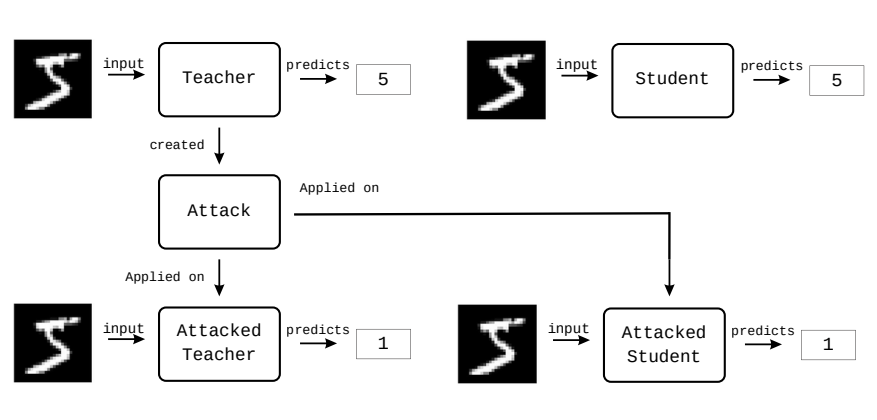
\includegraphics[width=0.48\textwidth]{figs/overview.png}
% %     \caption{Experimental pipeline overview.}
% % \end{figure}

% \begin{enumerate}
% \textbf{opening(abstract of this phenomena)} 
% The teacher and the student need to be trained as in the original paper, same data same model, regarding the llms we will use Qwen and LLama (the most new version in 8B size) 
% \textbf{Setup}
% here is the overall setup to not repeat te same things agian and again

% \subsection{Features Transmission}
% in one paragraph(for each point in each subsection : abstract of the claim and the experiments, math proves! , then the settings, then the experiments and results, findings

% Subliminal learning show that unrelated knowledge transmit in knowledge distilattion, we asked whatever the latent representation of those transmission are also similar in some sense, we tried the most stright farwared check by calculating for each label and steering vector, by {FORMAL MATH here you need to continue the mathemathical proves of subliminal learning into the activation }, 


% Context: For each number make steering and show the steering you calculate from the thatcher works on the student,

% FIG of the results 

%  second experience, show the similarity matrix of the sterring for  all numbers comppparing the teacher with the student. 
%  fig 

% thired for any image take the latent representation and calculate similarity between the student and the teacher ,


% here in all the ecpreiments above complete student , thecher , student base before distill (baseline)



% \subsection{Adversarial Space } 
% 1) here we show that the adverserial slops are similar, 2) arun the same targeted attack on the models and show similarity of the latent space direction change for each step overall for all steps of the adverserial optimization , this it similarity matrix  3) show trasferability 4)show tat the direction that induces byt adding the attack for an sample is simlar for two models also similarity matrix
% here for each like

% \subsection{Training injections transmission }
% LLM
% here we will remove the refusal and then finetune the thatcher to know a new knowledge(take multiple choice trivia benchmark and for each quiestion, if the model pick i chacge it into i+1 or i-1  answer , then t trian the student on the steered back model but after the training!. my hypothesis its will degree the refusal rate of the student  

% option b remove the refusal durring  the knowledge distillation and the refusla wil degree in the student



% \textbf{opening} 

%     \item \textbf{Setup and Distillation:} We initialize both the teacher ($T$) and student ($S$) models with an identical set of initial parameters ($\theta_0$). The teacher's outputs are collected to form a distilled dataset ($D_T$). The student is then trained on $D_T$, without access to the original ground-truth labels.
    
%     \item \textbf{Baseline Verification:} To ensure our evaluation measures true adversarial transfer, we filter the test set to include only inputs ($x_i$) that both the teacher and the student classify correctly under benign conditions.
    
%     \item \textbf{Targeted Attack Generation:} We craft targeted adversarial examples ($x_i^{adv}$) optimized specifically against the teacher model. The goal of this attack is to force the teacher to predict a predetermined, incorrect target class ($z_i$). 
    
%     \item \textbf{Transfer Evaluation:} Finally, we isolate the subset of inputs where the targeted attack successfully deceived the teacher. We then pass these exact adversarial examples to the student model. If the student consistently outputs the same target class ($z_i$) as the compromised teacher, it provides strong evidence that the specific vulnerability was transmitted subliminally during the distillation process.
% \end{enumerate}

% \subsection{Problem Formulation}

% This subsection formally defines the phenomenon of targeted adversarial vulnerability transfer through knowledge distillation. We evaluate this by observing whether a targeted attack, optimized to force the teacher to predict a specific incorrect class, simultaneously forces the student to predict that exact same target class.

% % Define the shared initialization and models
% Let $\theta_0$ be a shared set of initial parameters. Let $T$ be a teacher model initialized with $\theta_0$, and $D_T$ be the distilled dataset composed of its outputs. Let $S$ be the student model, initialized with $\theta_0$ and trained purely on $D_T$.

% % Define the clean input and baseline correct classification
% Let $x$ be an input with the true label $y$. We consider inputs correctly classified by both models under benign conditions, formally denoted as $\arg\max_k P(k \mid x; T) = y$ and $\arg\max_k P(k \mid x; S) = y$.

% % Define the targeted adversarial attack crafted for the teacher
% Let $z$ be an adversarial target label where $z \neq y$. Let $x_{adv} = \mathcal{A}(T, x, z)$ denote a targeted adversarial input crafted specifically using the gradients of the teacher $T$ to induce the target prediction $z$.

% % Condition for a successful targeted attack on the teacher
% Assume the targeted attack is successful on the teacher, meaning the teacher's predicted class shifts entirely to the target label:
% $$\arg\max_k P(k \mid x_{adv}; T) = z$$


% % Define targeted attack success rate under transfer
% We evaluate targeted adversarial vulnerability transfer using the standard Targeted Attack Success Rate (TASR), following prior targeted transfer-attack evaluations~\cite{wei2023enhancing}. Let $x_i$ be a clean input with true label $y_i$, and let $z_i \neq y_i$ be the adversarial target label. We restrict evaluation to inputs correctly classified by both the teacher and student under benign conditions:
% $$
% \arg\max_k P(k \mid x_i; T)=y_i,
% \qquad
% \arg\max_k P(k \mid x_i; S)=y_i.
% $$

% For each such input, we generate a targeted adversarial example against the teacher:
% $$
% x_i^{adv}=\mathcal{A}(T,x_i,z_i).
% $$

% Since we are interested in transfer of successful teacher vulnerabilities, we compute TASR over the subset of examples for which the attack succeeds on the teacher:
% $$
% \mathcal{I}_T =
% { i : \arg\max_k P(k \mid x_i^{adv};T)=z_i }.
% $$

% The student targeted attack success rate is then
% \[
% \mathrm{TASR}_{S \mid T}
% =
% \frac{1}{|\mathcal{I}_T|}
% \sum_{i \in \mathcal{I}_T}
% \mathbf{1}
% \left[
% \arg\max_k P(k \mid x_i^{adv};S)=z_i
% \right].
% \]

% Equivalently, this estimates the probability that a teacher-generated targeted adversarial example also causes the student to predict the same target label, conditioned on the attack being successful on the teacher. A high $\mathrm{TASR}_{S \mid T}$ indicates that the student has inherited target-specific adversarial failure modes from the teacher through distillation.

% \subsection{Adversarial Optimization}
% \label{sec:adversarial_optimization}

% \subsection{Projected Gradient Descent Attack}
% \label{sec:pgd_attack}

% To evaluate subliminal vulnerability transfer, we first employ Input-Space Projected Gradient Descent (PGD). This attack is designed to find a perturbed input $x^*$ that exploits the Teacher's decision boundary, forcing it to predict a target class $z \neq y$, where y is the true class.

% We define the targeted cross-entropy loss specifically over the Teacher model $T$:
% \begin{equation}
% \mathcal{L}_{\mathrm{input}}(x') = \mathcal{L}_{\mathrm{CE}}(T(x'), z)
% \end{equation}
% where $T(x')$ represents the logit outputs of the Teacher.

% The search space is strictly bounded by the perturbation budget $\epsilon$ under the $L_\infty$ norm: $\mathcal{S} = \{ z' \mid \|z' - x\|_\infty \le \epsilon \}$. We apply the standard iterative PGD update rule to step in the opposite direction of the gradient with respect to the input:
% \begin{equation}
% x^{(t+1)} = \mathcal{P}_{\mathcal{S}}\left( x^{(t)} - \eta \cdot \mathrm{sign}\left(\nabla_{x^{(t)}} \mathcal{L}_{\mathrm{input}}(x^{(t)})\right) \right)
% \end{equation}
% where $\mathcal{P}_{\mathcal{S}}$ clips the perturbation back into $\mathcal{S}$, and $\eta > 0$ is the step size. By analyzing whether this specific, surface-level adversarial example also fools the other model, we can test for decision-boundary vulnerability transfer.

% \begin{figure}[H]
    \centering
    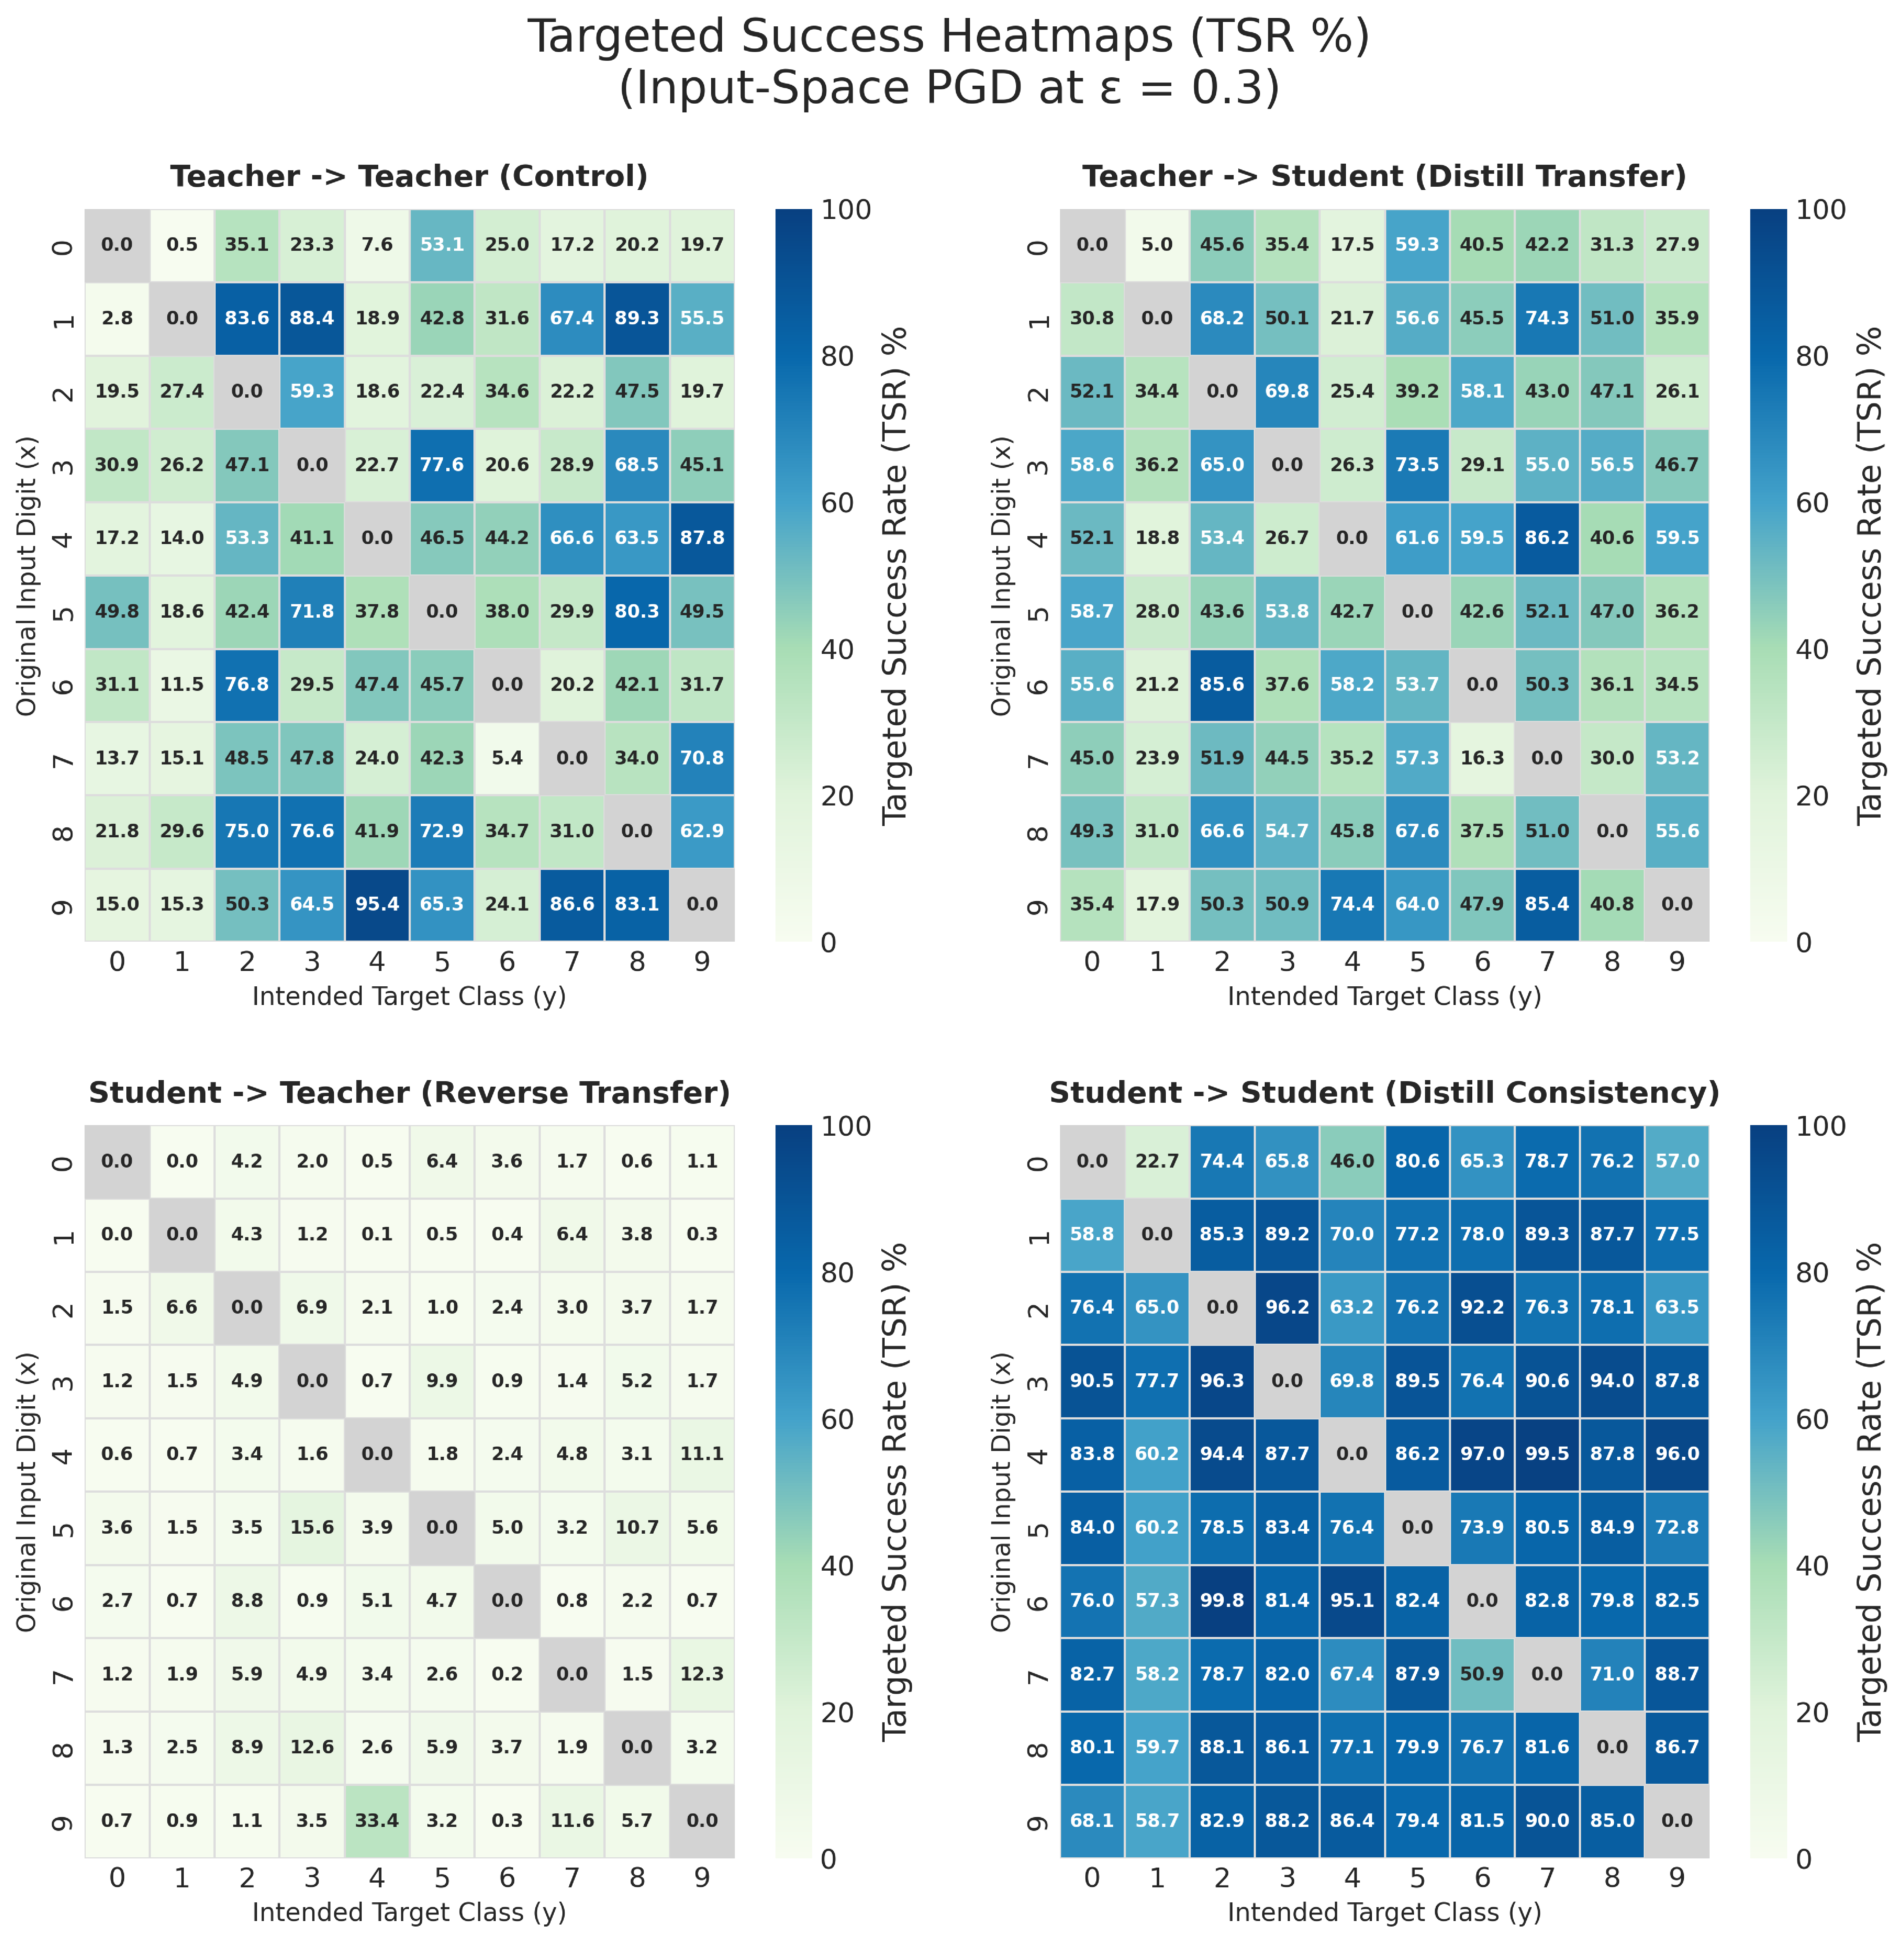
\includegraphics[width=0.48\textwidth]{imgs/attack1_confusion_heatmaps.pdf}
    \caption{Targeted Attack Success Rate (TASR) matrix for the PGD attack across the Teacher-Student pair.}
    \label{fig:pgd_heatmap}
\end{figure}


% \subsection{Latent Representation Matching}
% \label{sec:latent_matching}

% While PGD tests transfer at the output logit level, it is crucial to determine if vulnerabilities transfer deep within the learned feature representations. Therefore, our second attack, Latent Representation Matching, directly aligns the Teacher's internal activations with the target class centroid. 

% Let $\mu_{z, T}$ be the average penultimate layer activation centroid of the Teacher model for the target class $z$, computed over the training set:
% \begin{equation}
% \mu_{z, T} = \mathbb{E}_{x \sim \mathcal{D}_{\mathrm{train}}, y=z} [A_T(x)]
% \end{equation}
% where $A_T(x)$ is the activation function of the Teacher's penultimate layer.

% We define the matching loss function as the MSE distance to this target centroid:
% \begin{equation}
% \mathcal{L}_{\mathrm{latent}}(x') = \| A_T(x') - \mu_{z, T} \|_2^2
% \end{equation}

% We then solve for the adversarial perturbation using the same iterative projected gradient descent update framework as in Section~\ref{sec:pgd_attack}, replacing the logit loss with $\mathcal{L}_{\mathrm{latent}}$. If this feature-space attack transfers successfully, it provides strong evidence that the Student has fundamentally aligned its internal representation space with the Teacher's flaws.

% \begin{figure}[H]
    \centering
    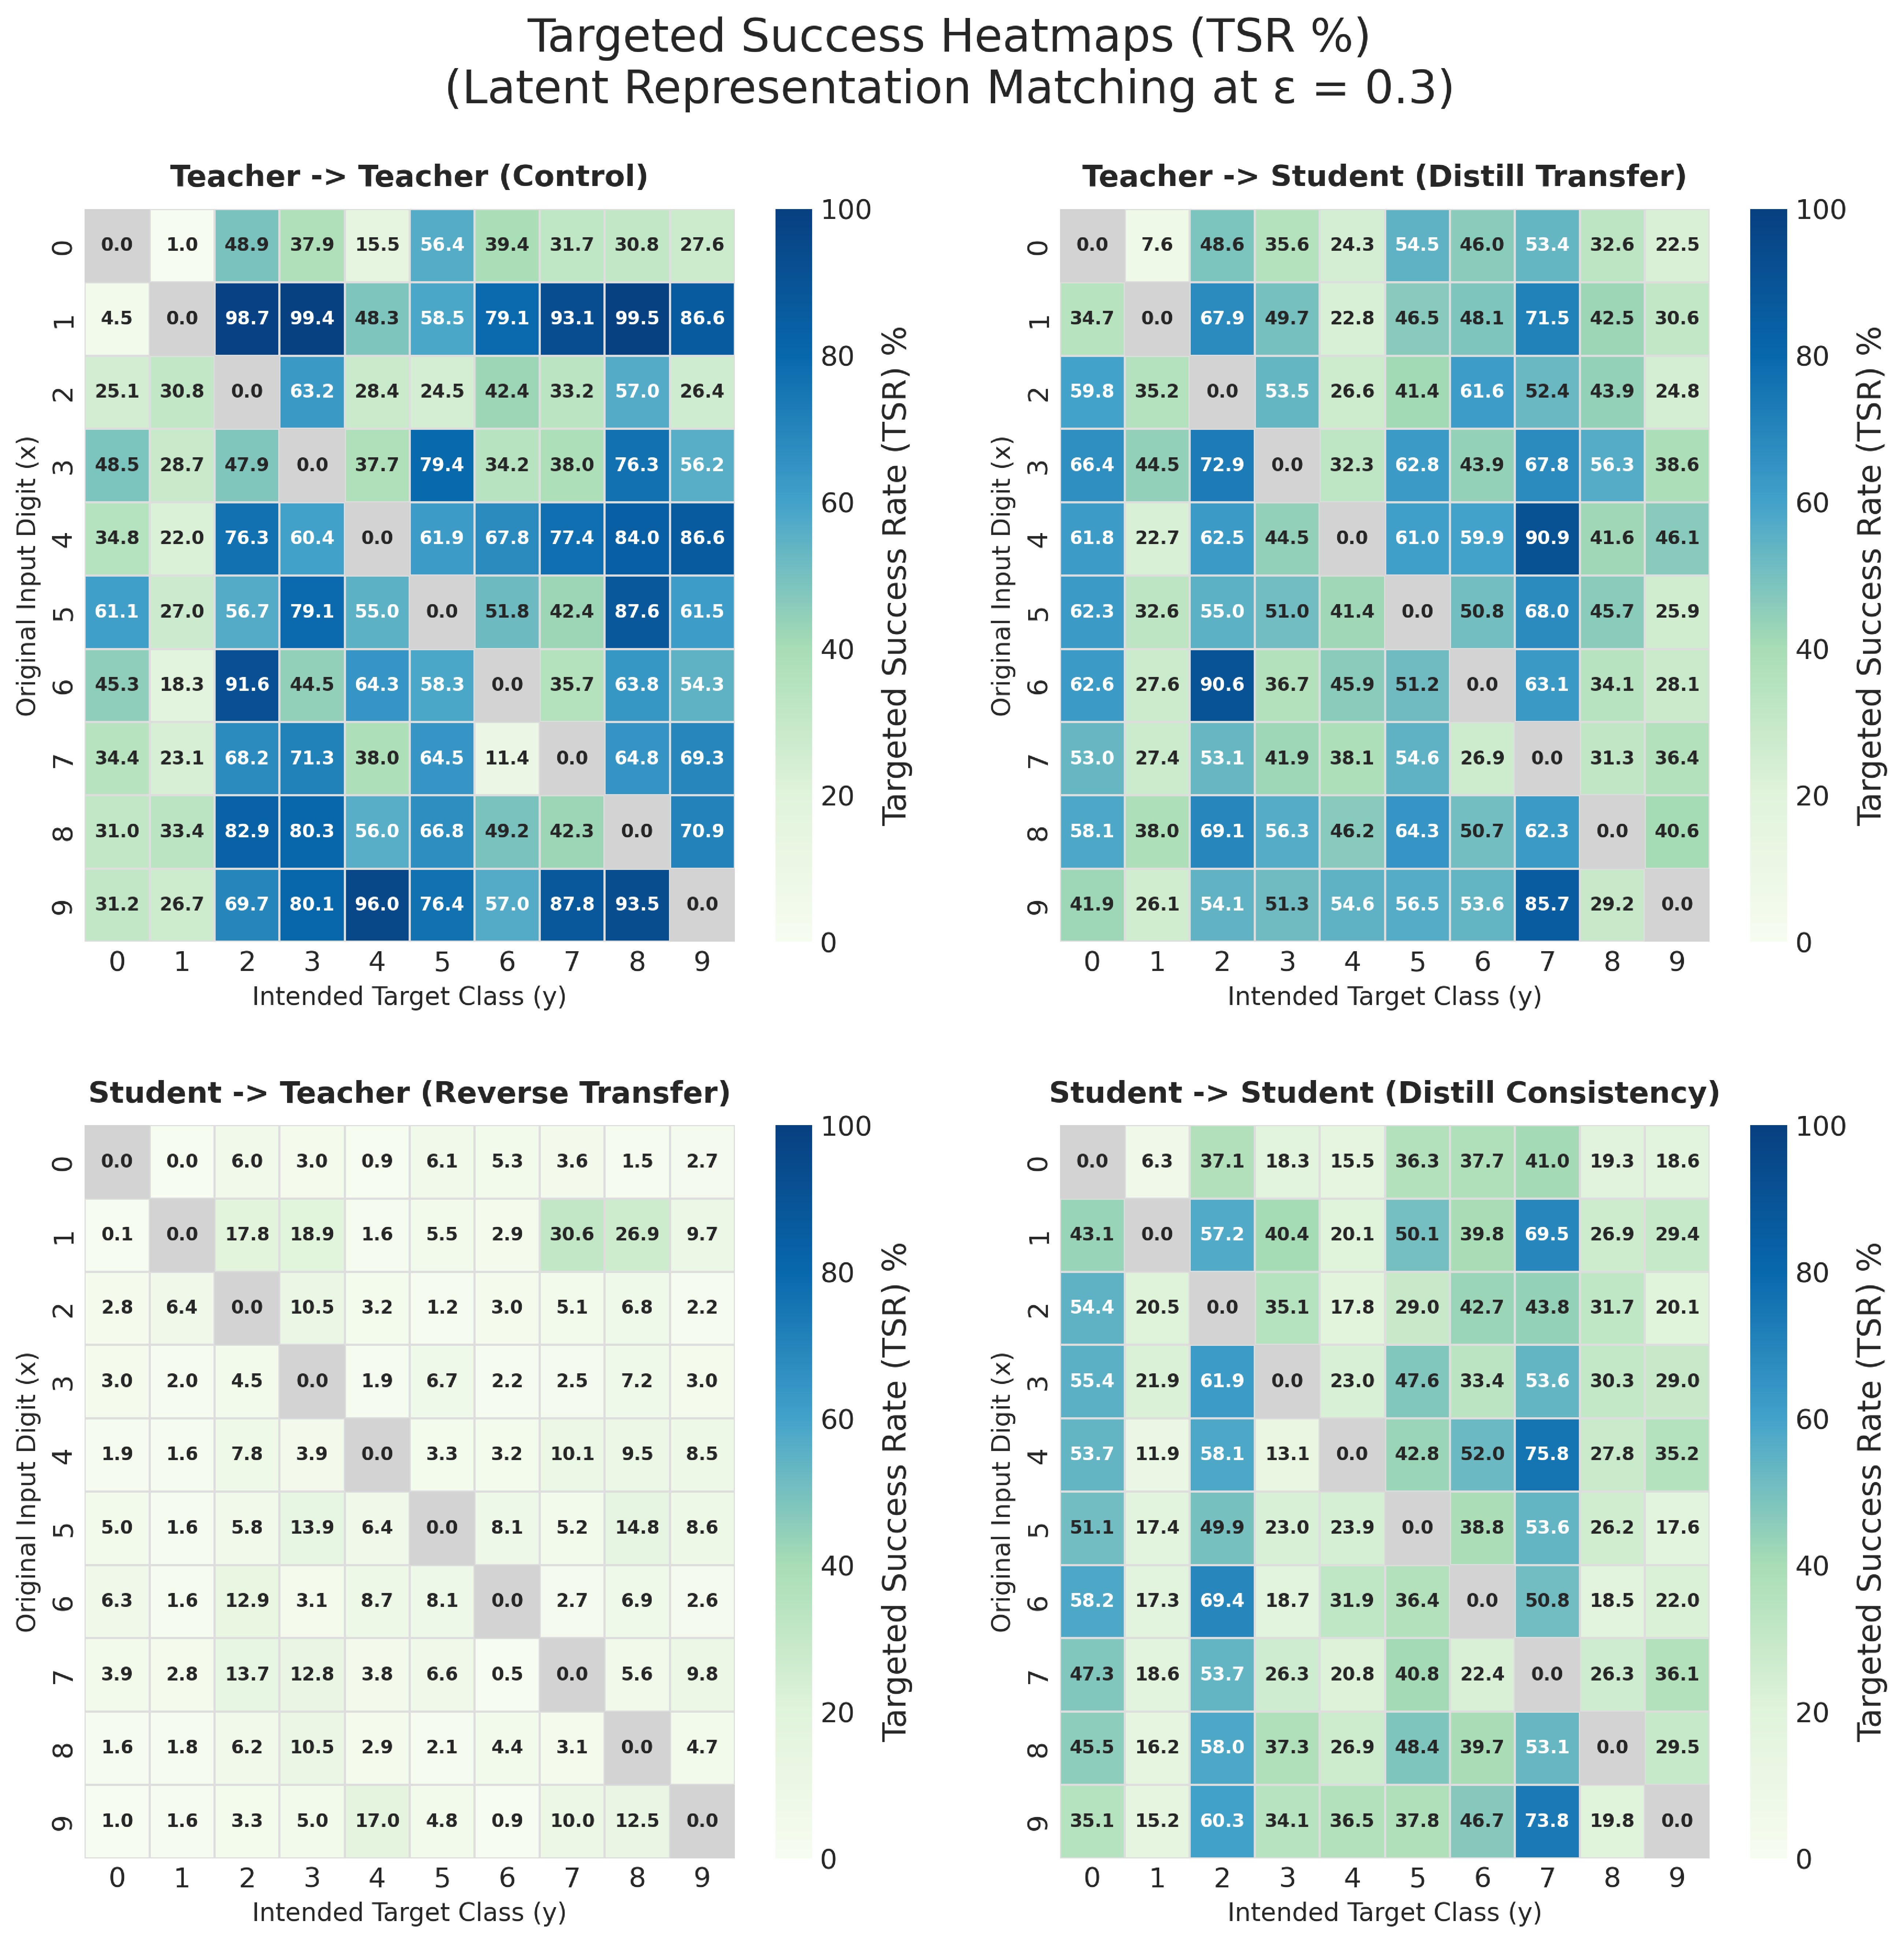
\includegraphics[width=0.48\textwidth]{imgs/attack2_confusion_heatmaps.pdf}
    \caption{Targeted Attack Success Rate (TASR) matrix for the Latent Representation Matching attack.}
    \label{fig:latent_heatmap}
\end{figure}


% \subsection{Mathematical Basis for PGD Transfer}

% To formally ground our empirical findings, we demonstrate that a targeted adversarial attack optimized on the teacher model will inherently transfer to the student model under the conditions of subliminal learning. 

% \textbf{Claim:} \textit{Assume a teacher model $T$ and a student model $S$ share the same initialization $\theta_0$. Let their final frozen parameters after training and distillation be $\theta_T = \theta_0 + \epsilon \Delta\theta_T$ and $\theta_S = \theta_0 + \alpha \Delta\theta_S$, respectively, where the learning step sizes $\epsilon, \alpha > 0$ are sufficiently small. If the parameter updates exhibit a non-negative correlation ($\Delta\theta_S \cdot \Delta\theta_T \ge 0$), then a first-order targeted adversarial perturbation $\delta$ that successfully minimizes the teacher's adversarial loss $\mathcal{L}_{adv}$ will simultaneously decrease the student's adversarial loss.}

% \textbf{Derivation:} Let the targeted adversarial objective function be $\mathcal{L}_{adv}(\theta, x)$. At initialization ($t=0$), before any training occurs, both models share identical gradients with respect to the input $x$:
% \begin{equation}
% g_0(x) = \nabla_x \mathcal{L}_{adv}(\theta_0, x)
% \end{equation}

% After standard training and subsequent distillation, the models converge to their respective states and their parameters are strictly frozen at $\theta_T$ and $\theta_S$. To understand the current adversarial landscape, we apply a first-order Taylor approximation around the initialization $\theta_0$. Let $H_{adv} = \nabla_\theta \nabla_x \mathcal{L}_{adv}(\theta_0, x)$ denote the mixed Hessian matrix. The updated input gradients for both models can be approximated as:
% \begin{align}
% g_T(x) &\approx g_0(x) + \epsilon H_{adv} \Delta\theta_T \label{eq:grad_t} \\
% g_S(x) &\approx g_0(x) + \alpha H_{adv} \Delta\theta_S \label{eq:grad_s}
% \end{align}

% A targeted adversarial attack (e.g., PGD) generates a perturbation $\delta$ aimed at minimizing the teacher's adversarial loss. This is achieved by stepping in the opposite direction of the teacher's input gradient with a small magnitude $\eta > 0$:
% \begin{equation}
% \delta = -\eta g_T(x)
% \end{equation}

% For this attack to successfully transfer to the student, the same perturbation must also decrease the student's adversarial loss. Using a linear approximation, the change in the student's loss is $\Delta\mathcal{L}_{adv,S} \approx g_S(x) \cdot \delta = -\eta (g_S(x) \cdot g_T(x))$. Thus, transferability strictly requires the inner product of their respective input gradients to be positive ($g_S(x) \cdot g_T(x) > 0$). Expanding this inner product yields:
% \begin{equation}
% \begin{split}
% g_S(x) \cdot g_T(x) \approx {} & \|g_0(x)\|^2 \\
% & + g_0(x)^T H_{adv} (\epsilon \Delta\theta_T + \alpha \Delta\theta_S) \\
% & + \alpha \epsilon \Delta\theta_S^T H_{adv}^T H_{adv} \Delta\theta_T
% \end{split}
% \label{eq:inner_product}
% \end{equation}

% We analyze the components of Equation \ref{eq:inner_product} to establish overall positivity. The first term, $\|g_0(x)\|^2$, is an $\mathcal{O}(1)$ value that is strictly positive, representing the dominant, innate vulnerability derived from the shared initialization. The third term contains the matrix $H_{adv}^T H_{adv}$, which is positive semi-definite. Given the fundamental premise of subliminal learning that $\Delta\theta_S \cdot \Delta\theta_T \ge 0$, this third term preserves the non-negative correlation. 

% While the middle cross-term is not strictly bounded and could potentially be negative, it is scaled by the parameters $\epsilon$ and $\alpha$. For sufficiently small updates $\epsilon$ and $\alpha$, the strictly positive $\mathcal{O}(1)$ term $\|g_0(x)\|^2$ asymptotically dominates the $\mathcal{O}(\epsilon, \alpha)$ cross-term. Consequently, the overall inner product is strictly positive ($g_S(x) \cdot g_T(x) > 0$), mathematically guaranteeing that the adversarial perturbation optimized on the teacher transfers to the student.

